% !TEX root = ../../main.tex
\chapter{Analysis Strategy}
\label{ch:analysisStrategy}
As motivated in~\Ch{\ref{ch:limitations}}, the boosted diboson resonance is a valuable probe of BSM physics. The semi-leptonic final state capitalizes on the properties of both hadronic and leptonic decays of weak bosons. In a $pp$ collider, the presence of an isolated high energy lepton in conjunction with \MET is a discerning feature that is useful for rejecting many QCD background processes. Requiring the other boson to decay hadronically takes advantage of a larger branching ratio, while mitigating the signal loss associated with the signal efficiencies of large-R jet boson tagging (\Sect{\ref{ch:objectReconstruction:larger}}).

In~\Sect{\ref{ch:analysisStrategy:evt_top}}, the boosted regime and the event topology of the search is described. The main SM background processes are detailed in~\Sect{\ref{ch:analysisStrategy:bkgs}}. Finally, the estimation of these SM backgrounds, as well as the benchmark signal models, through the use of Monte Carlo simulations is outlined in~\Sect{\ref{ch:analysisStrategy:sig_bkg_model}}. 

%
\section{Event Topology}
\label{ch:analysisStrategy:evt_top}
When hadronically decaying objects produced at the LHC have large transverse momentum, $\pt$, with respect to their rest mass, their decay products in the detector are very collimated, and they are referred to as boosted objects~\cite{lhc_boosted}. The search focuses on a heavy resonance decaying to a pair of boosted weak bosons: a $W$ boson decaying leptonically and either a $W$ or $Z$ boson decaying hadronically. The leptonically decaying $W$ is reconstructed as an isolated electron or muon, with a neutrino identified as \MET. The search considers topologies where the two quarks in the hadronic $W/Z$ decay cannot be separately resolved with the standard small-R jet reconstruction. Instead, they are reconstructed as a single boosted large-R jet with distance parameter $R=1.0$. 

%wrap was here

For diboson resonances produced just above threshold approximately at rest, the two decaying daughter bosons will have nearly equal \pT, as expressed in~\Eqn{\ref{eq:pt_larger}}. For each boson, the distance between the decay products is shown in~\Eqn{\ref{eq:dr_larger}}~\cite{LargeRjet_kin}. 
\begin{eqnarray}
\pt(V)&\simeq& m(WV)/2 \label{eq:pt_larger} \\
\Delta R(q,q)&\simeq&2m(V)/\pt(V) \label{eq:dr_larger}
\end{eqnarray}
When this separation becomes comparable to the distance parameter of reconstructed small-R jets ($R=0.4$), the reconstructed jets will partially or fully overlap, leading to degraded reconstruction efficiency and energy reconstruction. \Eqn{\ref{eq:dr_larger}} shows that, for SM weak bosons with $\pT(V)\simeq 200\,\GeV$, most of the hadronic activity can be recovered by the large-R jet. 
\begin{wrapfigure}{r}{.61\textwidth}
	\begin{center}
		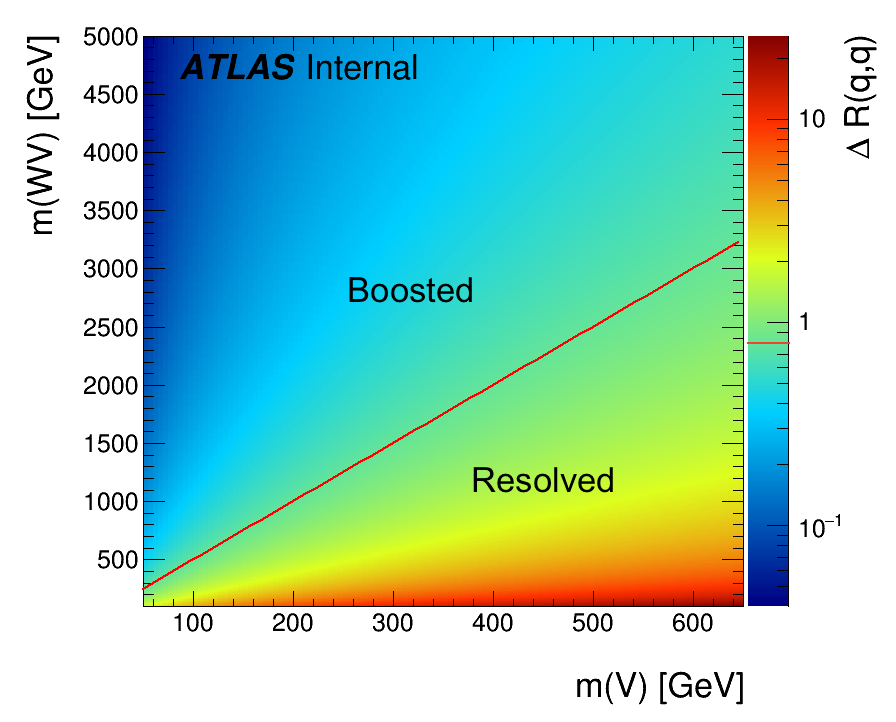
\includegraphics[width=.6\textwidth]{figures/AnalysisStrategy/h_boosted_resolved_2}
		\caption[Boosted and resolved regimes]{Representation of the boosted and resolved regimes as a function of $\Delta R(q,q)$ between the two quarks in the large-R jet.}
		\label{fig:boosted_regime}
	\end{center}
\end{wrapfigure}
For weak bosons with $\pT(V)\simeq 200\,\GeV$, this corresponds approximately to resonances with $m(WV)>500\,\GeV$. In \Fig{\ref{fig:boosted_regime}}, the boosted and resolved regimes are shown, separated by $\Delta R(q,q)\simeq 0.8$ between the two quarks in the hadronically decaying boson.  The angular separation of the quarks in the hadronically decaying $W$ boson from a simulated HVT $Z'$ signal (\Sect{\ref{ch:analysisStrategy:sig_bkg_model}}) for several mass points are shown in \Fig{\ref{fig:dr_qq}}. 


\begin{figure}[t!bh]
	\begin{center}
		\subfloat[]{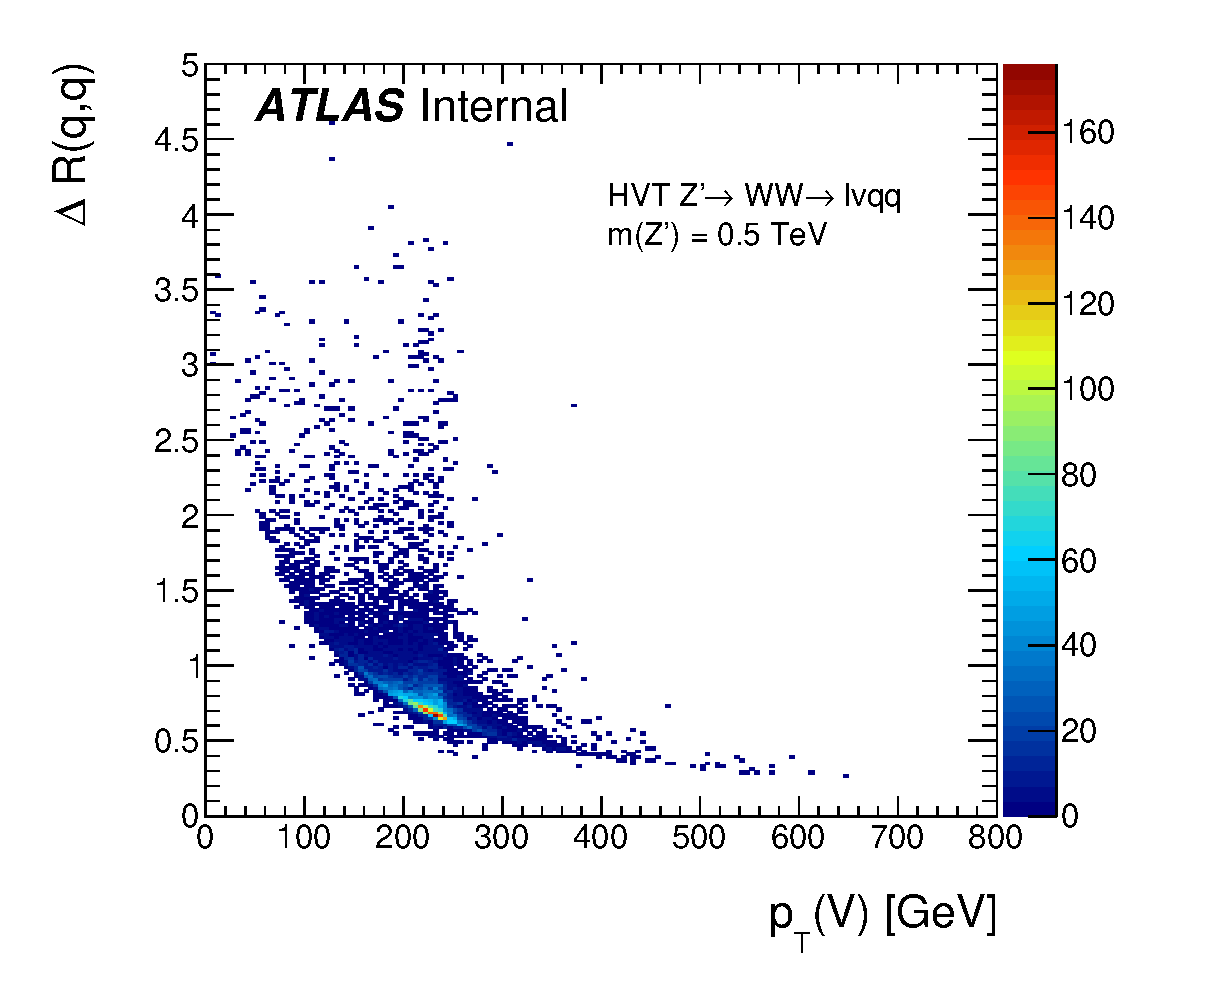
\includegraphics[width=.5\linewidth]{figures/AnalysisStrategy/h_DR_qq_W_500GeV}\label{fig:dr_qq_a}}
		\subfloat[]{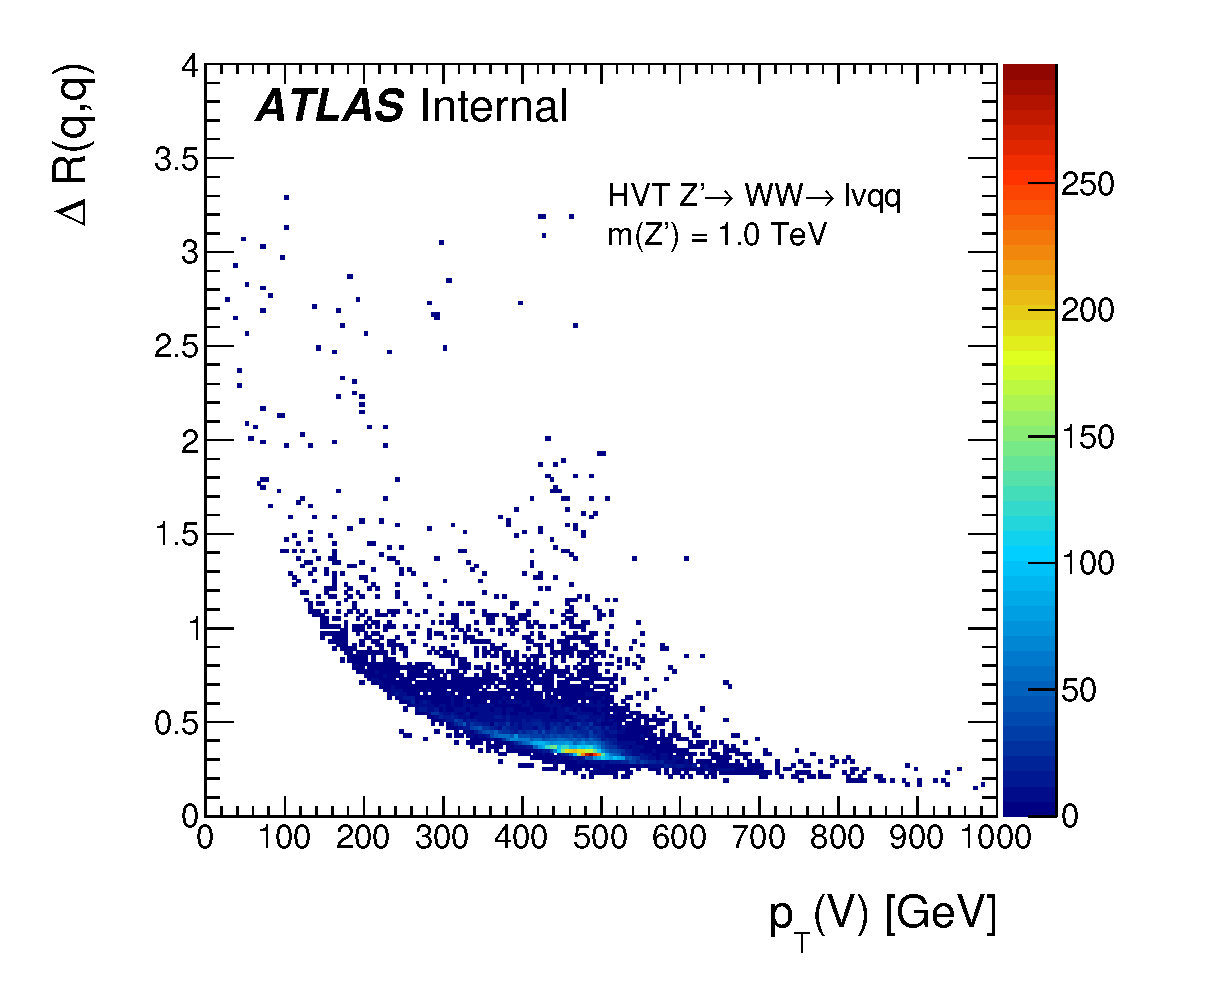
\includegraphics[width=.5\linewidth]{figures/AnalysisStrategy/h_DR_qq_W_1000GeV}\label{fig:dr_qq_b}}\\
		\subfloat[]{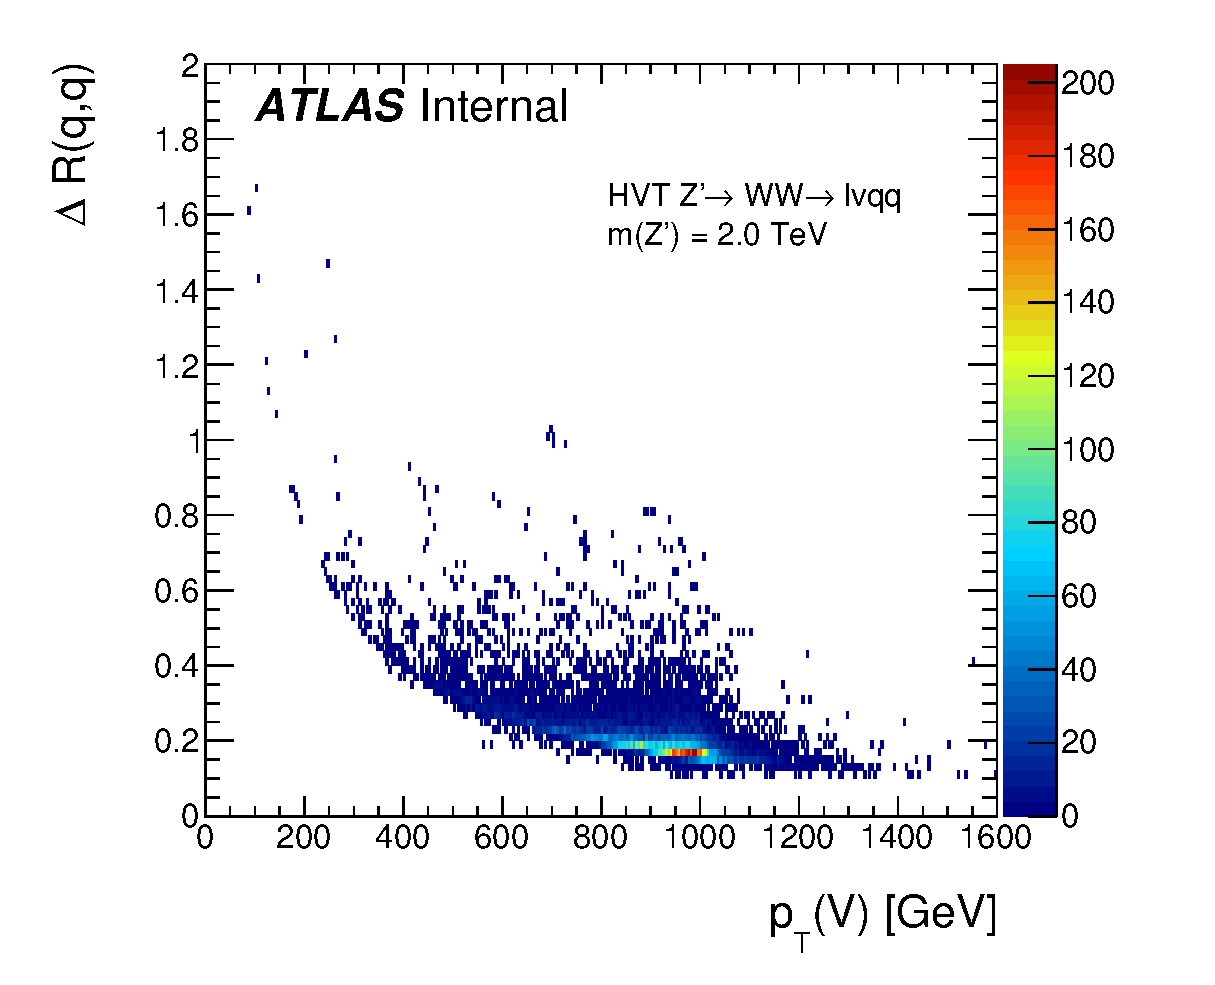
\includegraphics[width=.5\linewidth]{figures/AnalysisStrategy/h_DR_qq_W_2000GeV}\label{fig:dr_qq_c}}
		\subfloat[]{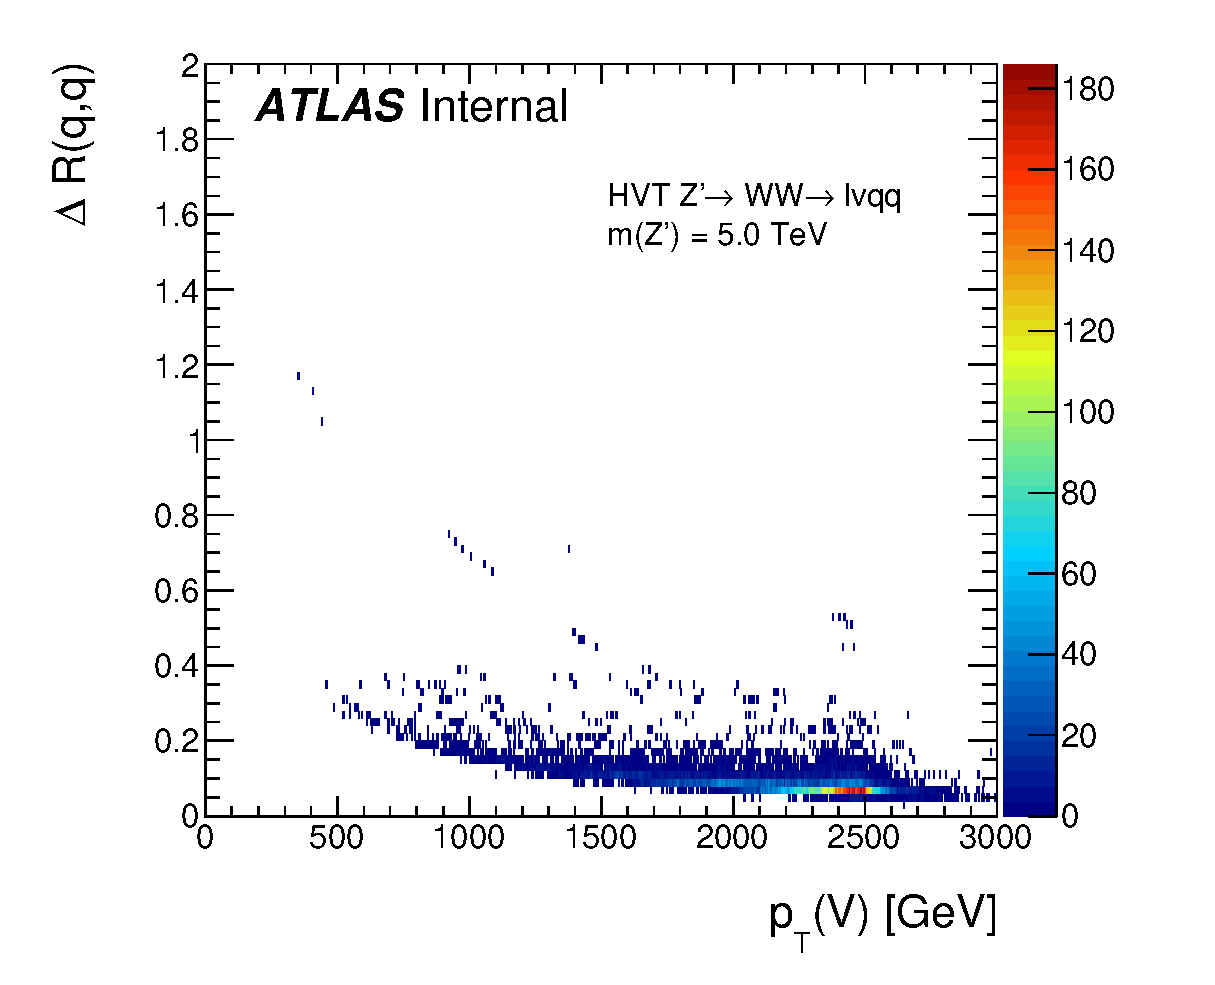
\includegraphics[width=.5\linewidth]{figures/AnalysisStrategy/h_DR_qq_W_5000GeV}\label{fig:dr_qq_d}}\\
		\caption[Separation of quarks as function of boson \pt]{Distribution of $\Delta R(q,q)$ vs $\pt(V)$ for HVT $Z'$ signal masses of \protect\subref{fig:dr_qq_a} 500 GeV, \protect\subref{fig:dr_qq_b} 1.0 TeV, \protect\subref{fig:dr_qq_c} 2.0 TeV, and \protect\subref{fig:dr_qq_d} 5.0 TeV.}
		\label{fig:dr_qq}
	\end{center}
\end{figure}


The search is split according to the signature of the production mechanism. In VBF production, the initial state quarks radiating vector bosons characteristically  hadronize with a large separation in $\eta$. These events are distinguished from gluon-gluon fusion and quark-quark fusion production by the presence of two additional small-R jets ($R=0.4$). The two event topologies of this analysis are depicted in~\Fig{\ref{fig:event_topology}}.

\begin{figure}[tb]
\begin{center}
\subfloat[]{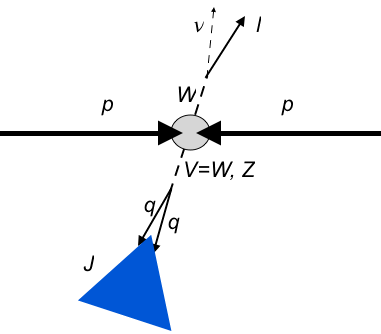
\includegraphics[width=0.49\textwidth]{figures/AnalysisStrategy/event_topology}\label{evt_topology:a}}\hfill
\subfloat[]{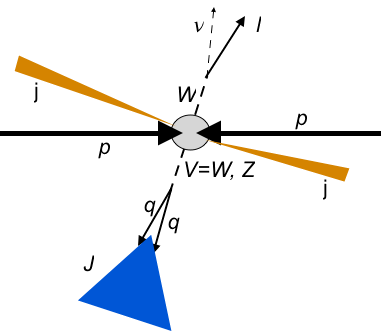
\includegraphics[width=0.49\textwidth]{figures/AnalysisStrategy/vbf_topology}\label{evt_topology:b}}
\caption[Diagram of event topologies]{The event topologies for \protect\subref{evt_topology:a} quark-quark fusion or gluon-gluon fusion, and \protect\subref{evt_topology:b} vector boson fusion (VBF). In both topologies, the heavy resonance decays to a central $W$ boson, further decaying leptonically ($W\ra \ell \nu$), and a central $V=W, Z$ further decaying hadronically ($W, Z\ra qq$). The neutrino, $\nu$, in the leptonic decay is reconstructed as missing transverse energy, $\MET$, while the hadronically decaying $V$ is reconstructed as a single large-R jet ($R=1.0$), denoted by $J$. In the case of VBF, two small-R jets ($R=0.4$) with a large separation are also present.}
\label{fig:event_topology}
\end{center}
\end{figure}




%
\section{Main Backgrounds}
\label{ch:analysisStrategy:bkgs}
In the SM, there are various processes which can produce or be reconstructed as the same final state as a semi-leptonic diboson resonance. In order to make an accurate interpretation of the data, these backgrounds must be understood and estimated. Those backgrounds which reproduce the exact final state ($\ell\nu qq$) are called irreducible backgrounds, and cannot be completely eliminated by improved selections. Other backgrounds which are reconstructed as the same final state, due to detector and reconstruction inefficiencies, are called reducible backgrounds, and can be significantly reduced with appropriate selections. Leading order Feynman diagrams of the main backgrounds considered in this search are depicted in~\Fig{\ref{fig:bkg_feyn_lo}}.

The most significant SM background in this analysis is the non-resonant production of a leptonically decaying $W$ boson ($W\ra\ell \nu$) in association with one or more quarks and gluons. The associated quarks and gluons hadronize and are reconstructed as jets; thus, this background is denoted by \Wjets. The QCD jets in this background have a non-resonant mass spectrum, and a different substructure with respect to a hadronically decaying weak boson of the signal. By taking advantage of boson tagging techniques (\Sect{\ref{ch:objectReconstruction:larger}}), the contamination of this background can be reduced. 

The second largest SM background comes from non-resonant top-antitop quark pair production, denoted by \ttbar. The semi-leptonic final state can be reproduced through the decay $t\bar{t} \ra bW^+\bar{b}W^- \ra b\bar{b}l\nu q\bar{q}'$. A decay of a top quark to a lighter down-type quark ($s$, $d$) is strongly suppressed.
%($<10\,\%$).  Much smaller, should I find a number?
The \ttbar background is thus characterized by the presence of $b$-jets in association with the final state. The use of $b$-tagging (\Sect{\ref{ch:objectReconstruction:smallr}}) can improve \ttbar rejection if any $b$-jets lie outside the reconstructed large-R jet.  For both \Wjets and \ttbar backgrounds, the normalization is estimated in dedicated control regions, as described in~\Sect{\ref{ch:eventSelection:srcr}}, using a fit described in~\Ch{\ref{ch:stats}}. 

A single leptonically decaying $Z$ boson ($Z\ra \ell\ell$) in association with jets is also a SM background for the search, denoted by \Zjets. Unlike the \Wjets background, \Zjets can only reproduce the semi-leptonic final state if one of the leptons is incorrectly reconstructed, and is thus reducible. A strict requirement on the number of leptons in the final state can significantly reduce this background.

In addition to the production of a top-antitop quark pair, the electroweak production of a single top quark, denoted \Singlet, can reproduce the semi-leptonic final state. In the $s$-channel and $t-$channel production, the final state is reproduced if the top quark decays leptonically through a $W$ boson. In the $Wt$-channel, a top quark is produced in association with a $W$. As with \ttbar, detecting the presence of additional $b$-tagged jets can help reduce the \Singlet background.

Finally, the non-resonant SM production of two weak bosons, denoted by SM dibosons, must be estimated. 

The non-resonant QCD production of multiple jets (multijet) has an extremely large cross section. Contamination from this background can occur if some of the jets are incorrectly reconstructed as leptons or involve decays with non-prompt leptons, and the reconstructed \MET is too large from detector inefficiencies. Since the modeling of the multijet background is difficult, due to the large rejection rate of fake leptons, the multijet contribution is estimated with a data driven approach. A control region with an enhanced expected QCD contribution (looser lepton selection, low \MET) is used to extract the shape of the multijet distribution. By requiring $\MET>100\,\GeV$ and a cut on $\MET/\pT(W\ra e\nu)$ (\Ch{\ref{ch:event_selection}}), the multijet background can be effectively suppressed, and is estimated to have a negligible impact on this search. More details can be found in~\App{\ref{ch:qcd}}.

\begin{figure}[tbp]
\centering
\begin{minipage}{.32\linewidth}
	 \subfloat[]{
		\feynmandiagram [small, horizontal=a to b, tree layout] {
			a --[gluon, edge label =\(g\)] b,
			b -- [fermion, edge label=\(t\)] c,
			b -- [anti fermion, edge label=\(\bar{t}\)] d, 
			c -- [boson] c1 [particle=\(W^+\)],   
			c -- [fermion] c2 [particle=\(b\)],
			d -- [boson] d1 [particle=\(W^-\)], 
			d -- [anti fermion] d2[particle=\(\bar{b}\)],
		};\label{fig:bkg_feyn_lo:a}}
\end{minipage}
\begin{minipage}{.32\linewidth}
    \subfloat[]{
       \feynmandiagram [small, horizontal=i1 to f2] {
			i1 [particle=\(q\)] -- [fermion] a -- [gluon] f2 [particle={\(g\)}],
			a -- [fermion] b,
			i2 [particle=\(\bar{q}'\)] -- [anti fermion] b -- [boson] f1 [particle={\(W/Z\)}],
			i1 -- [draw=none] i2,
			f1 -- [draw=none] f2
		}; \label{fig:bkg_feyn_lo:b}} \\
	\subfloat[]{
 	   \feynmandiagram [small, horizontal=a to b] {
			i1 [particle=\(q\)] -- [fermion] a -- [fermion] i2 [particle={\(\bar{q}'\)}],
			a -- [boson, edge label={\(W, Z\)}] b,
			f1 [particle=\(W\)] -- [boson] b -- [boson] f2 [particle={\(Z, W\)}],
		}; \label{fig:bkg_feyn_lo:c}}    
\end{minipage}
\begin{minipage}{.32\linewidth}
    \subfloat[]{
       \feynmandiagram [small, horizontal=i1 to f2] {
			i1 [particle=\(b\)] -- [fermion] a -- [fermion] f2 [particle={\(t\)}],
			a -- [boson, edge label=\(W\)] b,
			i2 [particle=\(q\)] -- [fermion] b -- [fermion] f1 [particle={\(q'\)}],
			i1 -- [draw=none] i2,
			f1 -- [draw=none] f2
		}; \label{fig:bkg_feyn_lo:d}} \\
	\subfloat[]{
 	   \feynmandiagram [small, horizontal=a to b] {
			i1 [particle=\(b\)] -- [fermion] a -- [gluon] i2 [particle={\(g\)}],
			a -- [fermion] b,
			f1 [particle=\(W\)] -- [boson] b -- [fermion] f2 [particle={\(t\)}],
		}; \label{fig:bkg_feyn_lo:e}}    
\end{minipage}
\caption[Selected leading order Feynman diagrams for background processes]{Selected leading order Feynman diagrams for the main background processes considered in this search. \protect\subref{fig:bkg_feyn_lo:a} \ttbar (one $W$ decays leptonically) can be reduced by tagging $b$-jets, \protect\subref{fig:bkg_feyn_lo:b} \Wjets and \Zjets backgrounds can be reduced with the help of boson tagging in the large-R jet, \protect\subref{fig:bkg_feyn_lo:c} SM diboson production will have a non-resonant mass spectrum, \Singlet production in the \protect\subref{fig:bkg_feyn_lo:d} $t$-channel and \protect\subref{fig:bkg_feyn_lo:e} $Wt$-channel can be reduced by tagging $b$-jets.}
\label{fig:bkg_feyn_lo}
\end{figure}


%
\section{Signal and Background Modeling}
\label{ch:analysisStrategy:sig_bkg_model}
Monte Carlo (MC) techniques are used to simulate both signal and background processes, and to model the response of the ATLAS detector. MC generated events are then used to optimize the event selection, and to compare the collected data with the estimated SM background contributions. A full list of the signal and background MC samples used in this analysis is available in~\App{\ref{ch:samples}}.
% Do I need this? 
%Precise modeling of estimated background contributions is vital in order to maintain high sensitivity to new physics.

Proton collisions at the LHC involve both hard (perturbative QCD) and soft (non-perturbative QCD) processes. As such, the event generation procedure involves splitting the full calculation into several smaller stages with different methods of evaluation. The first ``matrix element'' step involves calculating the initial hard scattering process of a fixed number of incoming and outgoing partons, using perturbative methods at leading-order (LO), or next-to-leading order (NLO) in powers of $\alpha_s$, the strong coupling constant. The subsequent showering of the outgoing partons, and hadronization of the color connected constituents, is modeled next. Finally, the ``underlying event'' (UE), comprised of processes not originating from the hard scatter event, are modeled and overlaid on the event. This includes initial and final state radiation from the incoming and outgoing partons in the hard scatter event, and additional interactions of the fragments of the colliding protons.

For all simulated samples, \textsc{Pythia} 8.186~\cite{pythia8} is used to model additional inelastic $pp$ interactions in the same bunch crossing, denoted as pile-up (PU). These PU interactions are then overlaid on the generated events. The number of PU events is reweighted with the standard ATLAS ``PileupReweightingTool'' so that the distribution of the average number of interactions per bunch crossing, $\langle\mu\rangle$, in the MC samples matches that in data. The particles in the simulated events are then propagated through the detector using the \textsc{GEANT4}~\cite{geant4} based detector simulation. The standard ATLAS reconstruction software~\cite{atlas_sim} then produces an event output in the same format as data. Physics objects are created using the same algorithms described in~\Ch{\ref{ch:objreco}}.

%
\subsection{Monte Carlo Generators}
The collisions at the LHC often involve the associated production of multiple hard (high-\pT) jets. The task of modeling the hard jet multiplicity can be accomplished either at the matrix element evaluation stage, or the showering stage. \textsc{Pythia} and \textsc{Herwig++}~\cite{herwig} are general $2\ra2$ generators which calculate the hard scatter matrix element for exactly two incoming and two outgoing particles. Both are capable of also modeling the showering process, where additional hard jets can be created. \textsc{Powheg}~\cite{powheg, powhegbox} is also a $2\ra2$ matrix element generator, but must be interfaced with another generator to model the showering and hadronization. 

\textsc{Sherpa}~\cite{sherpa} and \textsc{MadGraph}~\cite{mg5_anlo} are $2\ra n$ generators. For these generators, events with the same jet multiplicity can be produced either at the matrix element stage, or showering stage. An ambiguity resolution procedure is defined in order to not double count events.  \textsc{Sherpa} uses its own showering simulation similar to \textsc{Pythia}.  \textsc{MadGraph} is useful for modeling new physics by configuring parameters of a new interaction Lagrangian.

In order to accurately model proton collisions at the LHC, MC generators use parton distribution functions (PDF). The PDFs describe the probability that a certain parton with a specified momentum fraction exists in the initial protons. The PDFs depend on the resolution scale, $Q^2$, of a virtual photon probing the structure of the proton. For low $Q^2$, the proton is dominated by gluons and $u$ and $d$ quarks, while at higher $Q^2$, anti-quarks and heavier flavor quarks begin to populate the proton. PDFs are determined by fitting a large amount of data from multiple experiments. In this analysis, the following PDF sets are used: \textsc{NNPDF2.3} LO and \textsc{NNPDF3.0} NNLO~\cite{nnpdf}, \textsc{CTEQ6L1} ~\cite{cteq6l}, and \textsc{CT10}~\cite{ct10}.
%\hlfix{UE tuning}{Should I talk about this?}

%
\subsection{Signal Modeling}
\label{ch:anstrat:sm}
The signal models considered in this analysis include a neutral, scalar heavy Higgs boson, two HVT models with $W'$ and $Z'$ bosons, and a spin-2 RS graviton. For all the benchmark signal models, samples are produced such that the $\ell\nu qq$ final state is selected at the generator level.

A neutral, scalar heavy Higgs boson is generated using \textsc{Poweheg-Box} v1 with the \textsc{CT10} PDF set. The ggF and VBF production channels are simulated separately~\cite{heavy_higgs_VBF,heavy_higgs_ggF}.  Showering, hadronization, and the UE are calculated with \textsc{Pythia}8.186 using the \textsc{CTEQ6L1} PDF set. The scalar is modeled in the narrow width approximation (NWA), where interference effects with the SM Higgs and SM diboson production are neglected. Samples are produced for resonance masses from 500\,\GeV\, to 3\,\TeV, with a width of $4\,\MeV$.  
%Include? -> UE with the \textsc{AZNLO} tune~\cite{aznlo}

Since the width of the HVT $W'$ and $Z'$ are less than the detector resolution, samples generated for the Model-A ($g_V=1$) interpretation are used for the Model-B ($g_V=3$) interpretation as well, with scaling applied to account for the difference in cross section. \textsc{MadGraph5\_aMC@NLO} v2.2.2 is used to produce the signal samples, while \textsc{Pythia}8.186 using the \textsc{NNPDF2.3} LO PDF set models the showering, hadronization, and UE. % Include? ->  UE with the A14 tune~\cite{pythia_tune}. 
Samples for the $q\bar{q}$ fusion (VBF) production channel are produced for resonance masses from 500\,\GeV\, to 5\,\TeV\,(4\,\TeV). Samples for the VBF production channel explicitly set the fermionic coupling of the new vector bosons to zero, $c_F=0$.

Signal samples for the bulk RS graviton, produced via ggF, are created using the same generators as for HVT. Samples are generated for resonance masses between 500\,\GeV\, and 5\,\TeV\, and $k/\overline{M}_{\textrm Pl}=1.0$. For $k/\overline{M}_{\textrm Pl}=0.5$, the graviton has a different width and an event reweighting is applied to the generated $k/\overline{M}_{\textrm Pl}=1.0$ samples. The shape reweighting is applied as a function of the resonance mass, calculated at the parton level.

%
\subsection{Background Modeling}
Both \Wjets and \Zjets ($V+$jets) are modeled with \textsc{Sherpa} v2.2.1 and the \textsc{NNPDF3.0} NNLO PDF set. To aid event generation speed, a simplified scale setting prescription is used in determining the multi-parton matrix elements. The samples are divided by $\textrm{max}(h_{\rm T},\pt(V))$, where $h_{\rm T}$ is the scalar sum of the \pt of the associated jets in the event. The samples are classified by the number of $b$ and $c$ quarks in the final state. Additional samples are produced using \textsc{MadGraph5\_aMC@NLO} v2.2.2 to estimate systematic uncertainties associated with $V+$jets production. The \textsc{MadGraph5} samples simulate showering, hadronization and the UE with \textsc{Pythia} 8.186 using the \textsc{NNPDF2.3} LO PDF set.
% Include? UE using the \textsc{A14} tune (for cross check samples)

Backgrounds from \ttbar (one is required to decay leptonically), and \Singlet production in the $s-$channel and associated $Wt$ channel are simulated with \textsc{Powheg-Box} v2 using the \textsc{CT10} PDF set. The EW $t-$channel single top quark production is simulated with \textsc{Powheg-Box} v1 using the  \textsc{CT10}4f PDF set. In this case, both the matrix element calculation and PDF set correspond to a fixed four flavor scheme. All top processes model showering, hadronization and the UE with \textsc{Pythia} 6.428 using the \textsc{CTE6QL1} PDF set. The top quark mass is explicitly set to 172.5\,\GeV\, in the simulation. High-\pt radiation is damped in \textsc{Powheg} by setting the parameter \textsc{Hdamp}$=m_t$ to ensure good agreement with data in this region~\cite{hdamp}. Showering and hadronization systematic uncertainties are estimated using additional \textsc{Powheg-Box} samples, where the showering is modeled with \textsc{Herwig++} 2.7.1.
%UE for syst uncer -> textsc{UEEE5}~\cite{ueee5} 

SM diboson samples ($WW, WZ, ZZ$) are generated with \textsc{Sherpa} v2.1.1 using the \textsc{CT10} PDF set, where one boson is required to decay leptonically and the other hadronically. Alternate samples to estimate systematic uncertainties are generated with \textsc{Powheg-Box} using the \textsc{CT10} PDF set, where the showering, hadronization and UE are modeled with \textsc{Pythia} 8.186 using the \textsc{CTE6QL1} PDF set.

Decays of the bottom and charm quark are simulated with \textsc{EvtGen} v1.2.0~\cite{evtgen}, except for samples generated with \textsc{Sherpa}.
Generators for all background processes use cross sections determined at next-to-next-to-leading order (NNLO)~\cite{single_diboson, rapidity_nnlo, ttbar_nnlo, top_pp_nnlo, singletop_nnll, singletop_twoloop}, with the exception of the diboson samples which use the NLO cross sections from the generator\footnote{
The $t\bar{t}$ cross section includes the re-summation of next-to-next-to-leading logarithmic (NNLL) soft gluon terms.
}. 

